\chapter{Advanced Use}\label{chap:advUse}

This chapter gathers several topics that are reserved to advanced user of Harmony. 

\section{Starting from scratch}\label{newAnalysis:fromScratch}

If for some inexplicable reason you want to create your analysis project from scratch, this section will guide you. The first step is to create a plug-in project for this analysis. Make a right-click on the \emph{Project Explorer} view and select \texttt{New $\rightarrow$ Project $\rightarrow$ Plug-in Project} and \emph{Next}. You a wizard similar to the one presented in figure \ref{fig:new-plug-in}. For demonstration purpose we will call it \texttt{dummy}. Set the target platform to use the Equinox OSGi framework and press \emph{Next}.

	\begin{figure}[H]
		\centering
		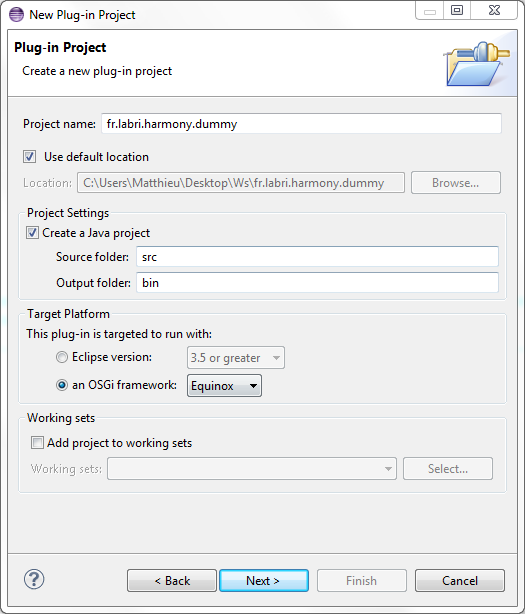
\includegraphics[width=.7\linewidth]{new-plug-in}
		\caption{First page of the plug-in wizard}
		\label{fig:new-plug-in}
	\end{figure}
	
Press next. You should now see the \texttt{Content} form as shown in figure \ref{fig:plug-in-content}, uncheck the \texttt{Generate an activator...} checkbox. Finally press \emph{Finish} to create your new project.

	\begin{figure}[H]
		\centering
		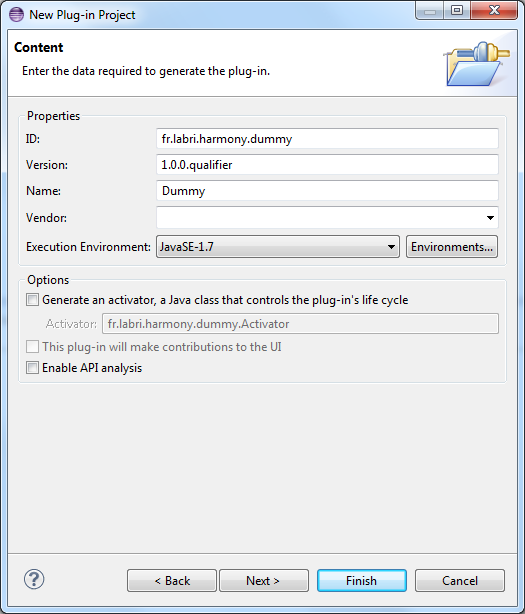
\includegraphics[width=.7\linewidth]{plug-in-content}
		\caption{First page of the plug-in wizard}
		\label{fig:plug-in-content}
	\end{figure}

In order for your analysis to use the harmony framework, you need to add the corresponding dependencies to your plug-in configuration. If it is not already the case open the \texttt{MANIFEST.MF} file located in the \texttt{META-INF} folder. Open the \texttt{Dependencies} tab, and add the following imported packages:

\begin{lstlisting}
fr.labri.harmony.core
fr.labri.harmony.core.analysis
fr.labri.harmony.core.config.model
fr.labri.harmony.core.dao
fr.labri.harmony.core.log
fr.labri.harmony.core.model
javax.persistence
\end{lstlisting}

You should obtain a configuration similar to the one presented in figure \ref{fig:harmony-dependencies}

	\begin{figure}[H]
		\centering
		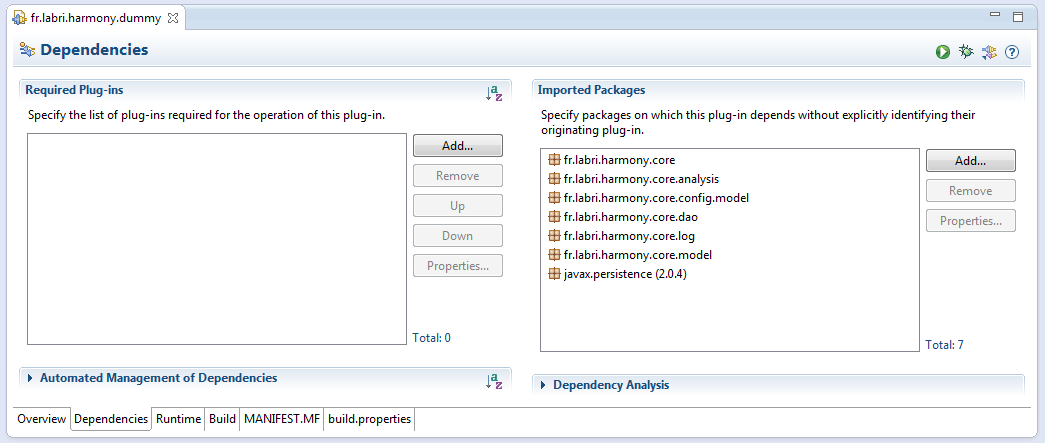
\includegraphics[width=\linewidth]{harmony-dependencies}
		\caption{First page of the plug-in wizard}
		\label{fig:harmony-dependencies}
	\end{figure}

You now have to add your analysis main class that will implement the \emph{AbstractAnalysis} class defined in the Harmony Core. To do so, use the Eclipse \emph{new class} wizard, and check the \texttt{Constructors from superclass} checkbox as shown in the figure \ref{fig:new-java-class}. 

	\begin{figure}[H]
		\centering
		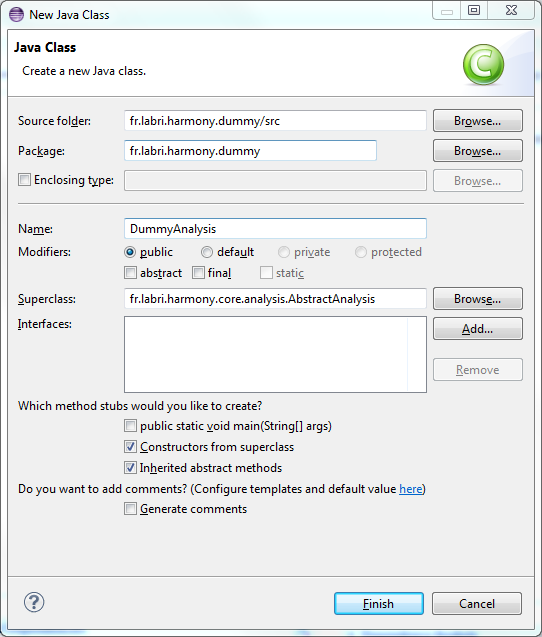
\includegraphics[width=.7\linewidth]{new-java-class}
		\caption{Creation of the main class of class of your analysis}
		\label{fig:new-java-class}
	\end{figure}

This is very important, as \textbf{both constructors from AbstractAnalysis are mandatory}. Also add as your superclass: \\ \emph{fr.labri.harmony.core.analysis.AbstractAnalysis}\\
Press \emph{Finish}. You should have something looking like the class presented in the listing \ref{code:dummyAnalysis}. The method \emph{runOn(Source src)} is where you must implement your analysis. Take a look at existing analyses for inspiration. Follow the same procedure as the one you have followed for importing the \emph{fr.labri.harmony.core} (see section \ref{sec:RunInEclipse}).

\includeSourceFile{resources/listings/DummyAnalysis.java}{DummyAnalysis lass}{code:dummyAnalysis}{java}

You now have a class that implements the analysis service so you need to inform the OSGi runtime about your implementation. Create an empty folder called \emph{OSGI-INF} at the root of your project. Then create a new component definition : make a right-click on your plug-in project and select \texttt{New $\rightarrow$ Component Definition}. Complete the form by taking example of the figure \ref{fig:new-component}, for example the component definition should be in the newly created  \emph{OSGI-INF} folder. Finally press \emph{Finish}.

	\begin{figure}[H]
		\centering
		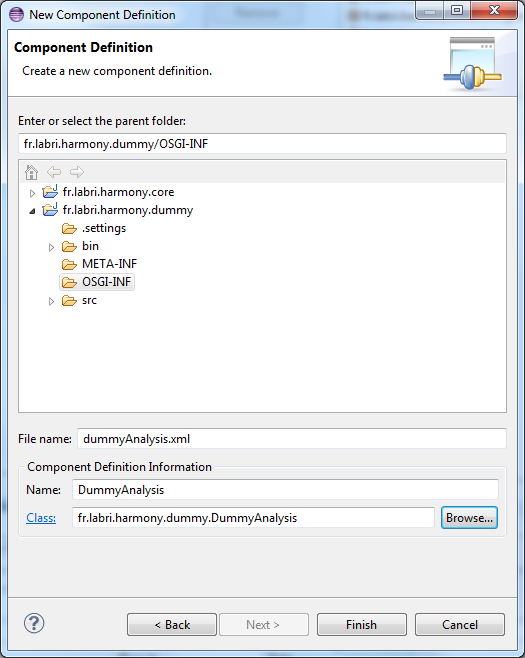
\includegraphics[width=.7\linewidth]{new-component}
		\caption{Wizard for creating a new component definition}
		\label{fig:new-component}
	\end{figure}
	
Open the newly created file and go the \emph{Service} tab as shown in the figure \ref{fig:provided-services}. Click on the \emph{Add} button of the \emph{Provided Services} section and select \texttt{fr.labri.harmony.core.analysis.Analysis}, press \emph{Ok}.
	
	\begin{figure}[H]
		\centering
		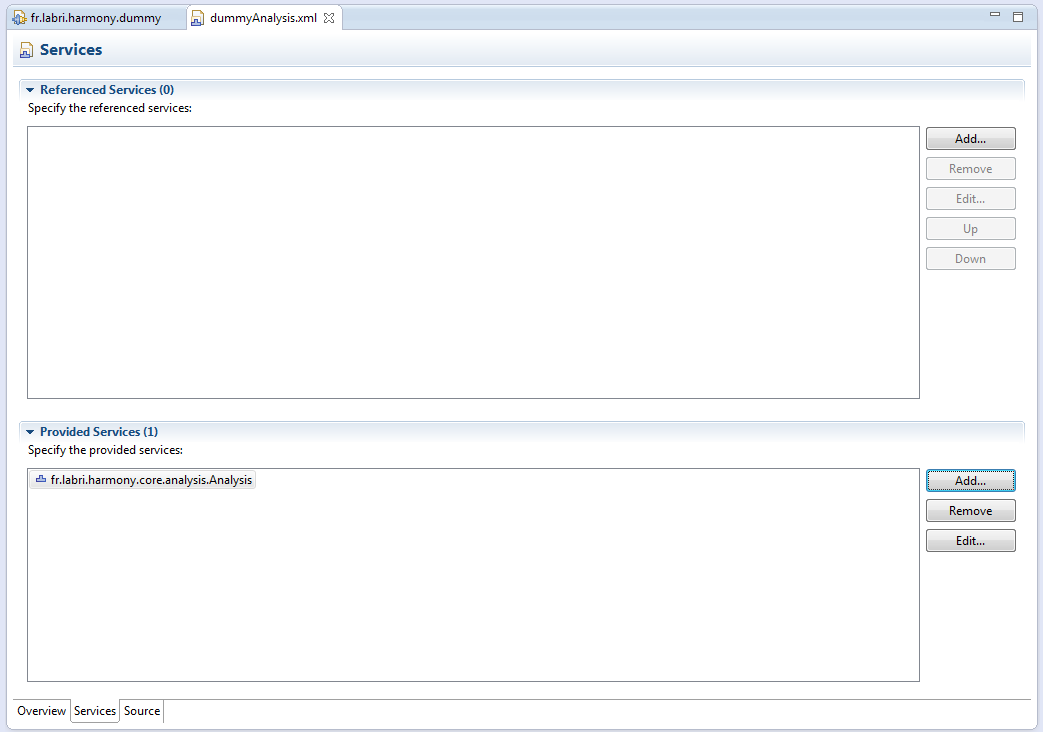
\includegraphics[width=\linewidth]{provided-services}
		\caption{Provided services}
		\label{fig:provided-services}
	\end{figure}
	
Your analysis project is now set up. You can run it by modifying your configuration files (see Chapter \ref{chap:configuration}) and your \emph{Run Configuration} (see Section \ref{sec:RunInEclipse}).